\setcounter{page}{1}
\section{行业情况}
\subsection{行业概述}
现阶段中国在线教育的宏观发展环境一片利好.移动化和网络化的生活习养成、教育需求的上升以及技术的更新迭代为中国在线教育的发展注入源源不断的动力.从需求端角度来讲,用户对线上教育的认可度不断提升,对线上教育的种类和深度提出了更高的要求,同时随着知识扁平化的出现,用户对教学有效和教学体验的要求也将进一步推动在线教育发展。从供给端角度来看,大部分教师、教育机构及知识甲等都承担着教育盈余输出的角色,线上教育平台能够从技术、运营、推广、生源等方面提供辅助,而教师或机构的入驻能够进一步吸引生源从而带动平台收入,形成共赢局面。
但在实际市场上来看,还没有一家公司能够做到对在线教育、知识付费领域的主导地位,只是在某些细分领域有相应的领域领先者。而在线教育、知识付费领域的市场是巨大的,而且在逐年增长的过程中。
\subsection{政策说明}
\subsubsection{资金扶持}\

2014 年起,启动北京地区高校大学生创业优秀团队评选,给予优秀创业团队( 企业) 最多20 万元资助,并优先入驻大学生创业园。首批103个大学生创业优秀团队扶持资金1300 万元。2015 年预计资助400个优秀团队,扶持资金3200 万元。开展“北京高校大学生创新、创意、创业实践项目”支持,计划支持100个左右大学生创业团队、400个左右大学生创新创意、创业实践团队。

设立北京青年创业小额贷款担保基金,推出10 万元以下初创型企业小额贷款和500 万元以下成长型企业小额贷款项目。将个体工商户小额担保贷款最高担保额度和享受财政贴息最高贷款额度提高至20 万元,将小微企业担保贷款最高担保额度和享受财政贴息最高贷款额度提高至100 万元。同时,符合条件的北京市合同期满未就业大学生村官和本市低保、低收入家庭高校毕业生不提供任何担保就申请贷款。

\subsubsection{创业载体建设}\

中国人民大学大学生创业园,凡为中国人民大学注册在校生、应届毕业生及已毕业(两年内)尚未就业的大学生,经中国人民大学在职教师推荐,均可申请入驻学生创业园,包括本科生、硕士生、博士生。

\subsubsection{创业教育培训}\

\paragraph{教育形式多种多样}\

先后在中国人民大学等7 所高校开设创业培训服务基地校,符合条件的高校毕业生可享受创业导师辅导。拥有北京市户籍的大学生可根据自身创业需求,到指定创业培训定点机构参加一次免费创业培训。

\paragraph{辅导专家团队不断组建}\

2009 年,北京首家“大学生创业指导中心”在北京交通大学挂牌。2014 年,启动北京高校示范性创业中心建设工作,用三年时间建设40个左右示范性高校创业指导中心。首批中国农业大学、首都师范大学等24所高校入选,分别给予50万元建设经费支持。

\paragraph{创新创业竞赛蓬勃发展}\

2000 年起,北京开始举办首都大学生创业计划竞赛,80 余所高校超过50 万大学生直接或间接参与创业竞赛活动,目前已举办8 届。2013 年起,每年举办北京市大学生创业设计竞赛,搭建大学生创业设计成果交流展示平台。2014 年,北京市大学生创业引领计划之“东升杯”大学生创业大赛正式启动,优胜者将可获得现金奖励、免费办公场所、全方位孵化服务等奖项,总价值200余万。(“互联网+“创业大赛。)

\subsection{用户人群}
用户人群标签:
\begin{figure}[H]
	\centering
	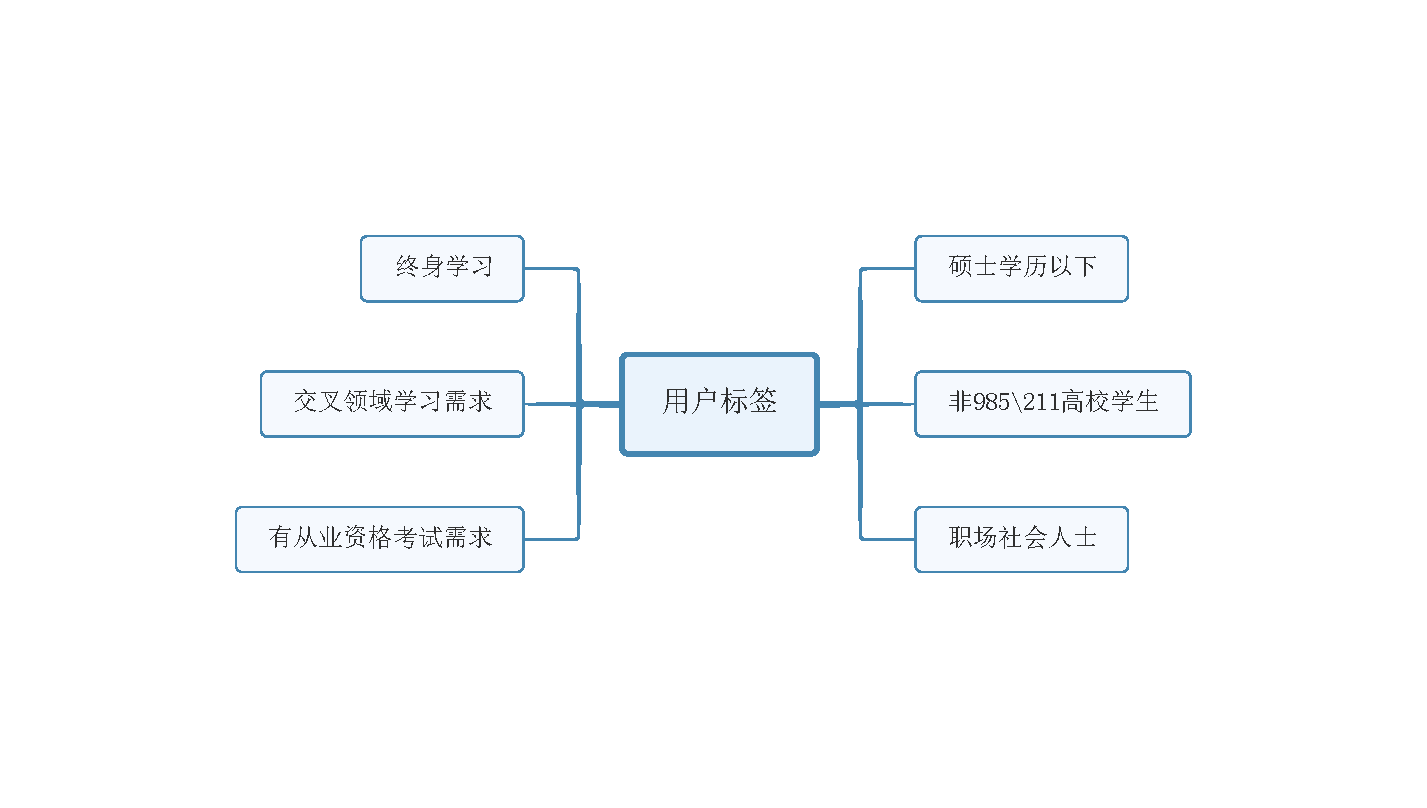
\includegraphics[width=0.9\columnwidth]{figures/user_label}
	%  \setlength{\abovecaptionskip}{0pt}
	%  \setlength{\belowcaptionskip}{-20pt}
	\caption{用户人群标签}
	\label{fg:user_label}
\end{figure}

\subsection{未来发展}
参考以下数据:
\begin{figure}[H]
	\centering
	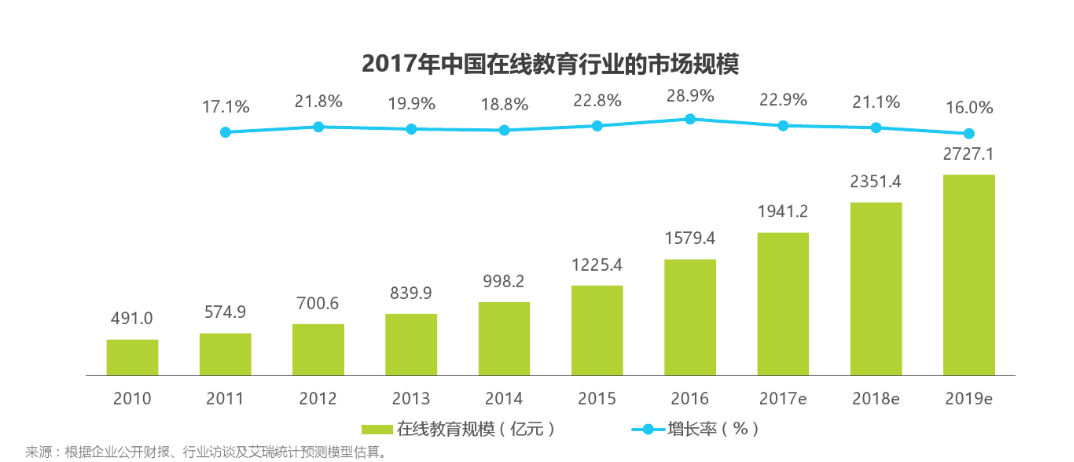
\includegraphics[width=0.9\columnwidth]{figures/2017online_education}
	%  \setlength{\abovecaptionskip}{0pt}
	%  \setlength{\belowcaptionskip}{-20pt}
	\caption{2017年在线教育行业的市场规模}
	\label{fg:2017online_education}
\end{figure}

\begin{figure}[H]
	\centering
	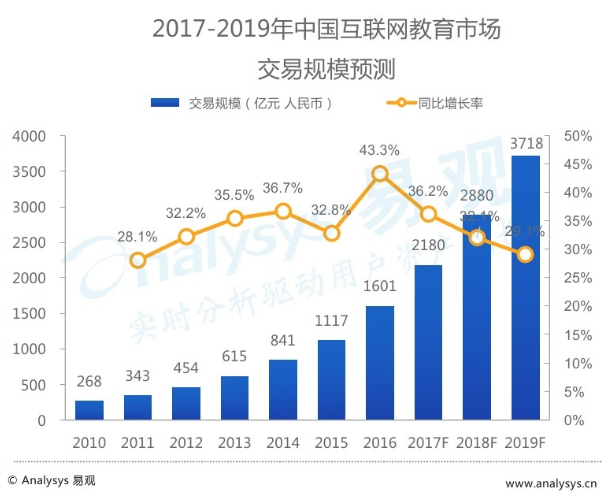
\includegraphics[width=0.9\columnwidth]{figures/2017_2019internet_education}
	%  \setlength{\abovecaptionskip}{0pt}
	%  \setlength{\belowcaptionskip}{-20pt}
	\caption{2017-2019年中国互联网教育市场交易规模预测}
	\label{fg:2017_2019internet_education}
\end{figure}

\begin{figure}[H]
	\centering
	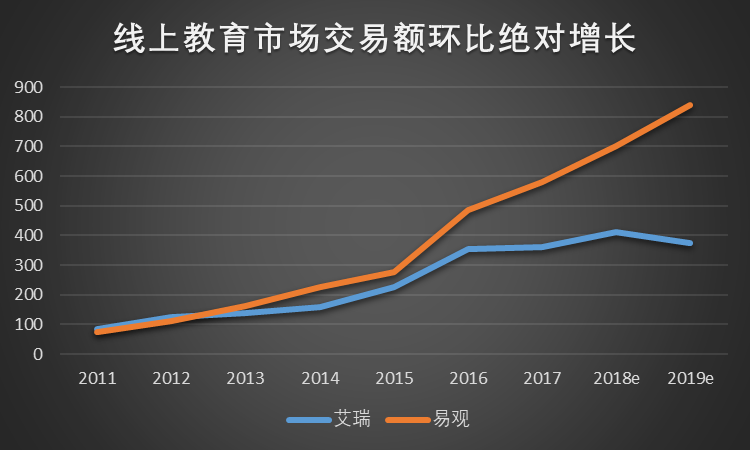
\includegraphics[width=0.9\columnwidth]{figures/online_education}
	%  \setlength{\abovecaptionskip}{0pt}
	%  \setlength{\belowcaptionskip}{-20pt}
	\caption{线上教育市场交易额环比绝对增长}
	\label{fg:online_education}
\end{figure}

\subsubsection{宏观环境利好}\

互联网+教育、教育信息化及AI+教育等利好政策频出;

网络经济上行,网络化和移动化生活习惯养成;

社会供需失衡,随着中产阶级崛起,人们付费意识觉醒,教育需求和教育消费迎来升级;

互动直播、大数据、人工智能等技术提升线上教育教学体验;

根据《新媒体蓝皮书:中国新媒体发展报告(2018)》,到2017年底,知识付费用户达到1.88亿人,比2016年增长了102.2%。而华菁证券的研报推断,到2020年知识付费将会有2亿人群、45%付费率、360元ARPU值,行业总收入规模达到320亿。

\subsubsection{知识需求端市场旺盛}\

在线教育用户规模持续扩张,在线教育的市场认可度逐渐提升,对线上课程的广度和内容深度要求提升;

终身学习和对交叉领域知识的需求增加测试用户需要学习的阶段不断延长;

用户重视学习的有效性,并对线上学习体验不断提出新的需求。

\subsubsection{知识供给端输出盈余}\

传统教师或中小型教育机构转型线上教育成本高且经验缺乏;
独立知识分享者可提供短平快的知识输出,但是在生源和推广方面有待加强。
















